% Created 2023-02-17 vie 11:04
% Intended LaTeX compiler: pdflatex
\documentclass[aspectratio=169, usenames,svgnames,dvipsnames]{beamer}
\usepackage[utf8]{inputenc}
\usepackage[T1]{fontenc}
\usepackage{graphicx}
\usepackage{longtable}
\usepackage{wrapfig}
\usepackage{rotating}
\usepackage[normalem]{ulem}
\usepackage{amsmath}
\usepackage{amssymb}
\usepackage{capt-of}
\usepackage{hyperref}
\usepackage{color}
\usepackage{listings}
\usepackage{mathpazo}
\usepackage{gensymb}
\usepackage{amsmath}
\usepackage{diffcoeff}
\usepackage{steinmetz}
\usepackage{mathtools}
\usepackage{fancyvrb}
\DefineVerbatimEnvironment{verbatim}{Verbatim}{fontsize=\tiny, formatcom = {\color{black!70}}}
\bibliographystyle{plain}
\usepackage{siunitx}
\sisetup{output-decimal-marker={,}}
\DeclareSIUnit{\watthour}{Wh}
\DeclareSIUnit{\wattpeak}{Wp}
\DeclareSIUnit{\watthour}{Wh}
\DeclareSIUnit{\amperehour}{Ah}
\usepackage{steinmetz}
\hypersetup{colorlinks=true, linkcolor=Blue, urlcolor=Blue}
\renewcommand{\thefootnote}{\fnsymbol{footnote}}
\parskip=5pt
\usepackage{tikz}
\usetheme{Boadilla}
\usecolortheme{rose}
\usefonttheme{serif}
\author{\href{https://oscarperpinan.github.io}{Oscar Perpiñán Lamigueiro}}
\date{}
\title{Variabilidad de la Potencia de una Central Fotovoltaica}
\subtitle{Energía Solar Fotovoltaica}
\institute[UPM]{Universidad Politécnica de Madrid}
\setbeamercolor{alerted text}{fg=blue!50!black} \setbeamerfont{alerted text}{series=\bfseries}
\AtBeginSubsection[]{\begin{frame}[plain]\tableofcontents[currentsubsection,sectionstyle=show/hide,subsectionstyle=show/shaded/hide]\end{frame}}
\AtBeginSection[]{\begin{frame}[plain]\tableofcontents[currentsection,hideallsubsections]\end{frame}}
\beamertemplatenavigationsymbolsempty
\setbeamertemplate{footline}[frame number]
\setbeamertemplate{itemize items}[triangle]
\setbeamertemplate{enumerate items}[circle]
\setbeamertemplate{section in toc}[circle]
\setbeamertemplate{subsection in toc}[circle]
\hypersetup{
 pdfauthor={\href{https://oscarperpinan.github.io}{Oscar Perpiñán Lamigueiro}},
 pdftitle={Variabilidad de la Potencia de una Central Fotovoltaica},
 pdfkeywords={},
 pdfsubject={},
 pdfcreator={Emacs 28.2 (Org mode 9.6)}, 
 pdflang={Spanish}}
\begin{document}

\maketitle

\section{Introducción}
\label{sec:orgce5f5b7}

\begin{frame}[label={sec:org29e0409}]{Los Sistemas Fotovoltaicos y la Red Eléctrica}
Los sistemas fotovoltaicos conectados a red alteran las condiciones de
funcionamiento habitual de la red.

\begin{center}
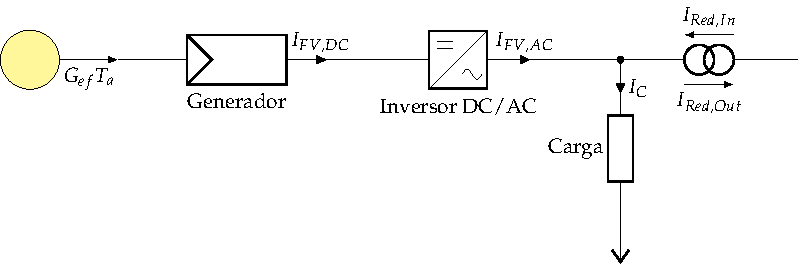
\includegraphics[width=\textwidth]{../figs/SFCR_bidireccional.pdf}
\end{center}
\end{frame}

\begin{frame}[label={sec:org184de90}]{Los Sistemas Fotovoltaicos y la Red Eléctrica}
\begin{itemize}
\item Posibilitan la bidireccionalidad del flujo de potencia, con los
consiguientes cambios en la tensión de los nodos, y en la corriente
conducida por las líneas y transformadores.
\end{itemize}

\begin{center}
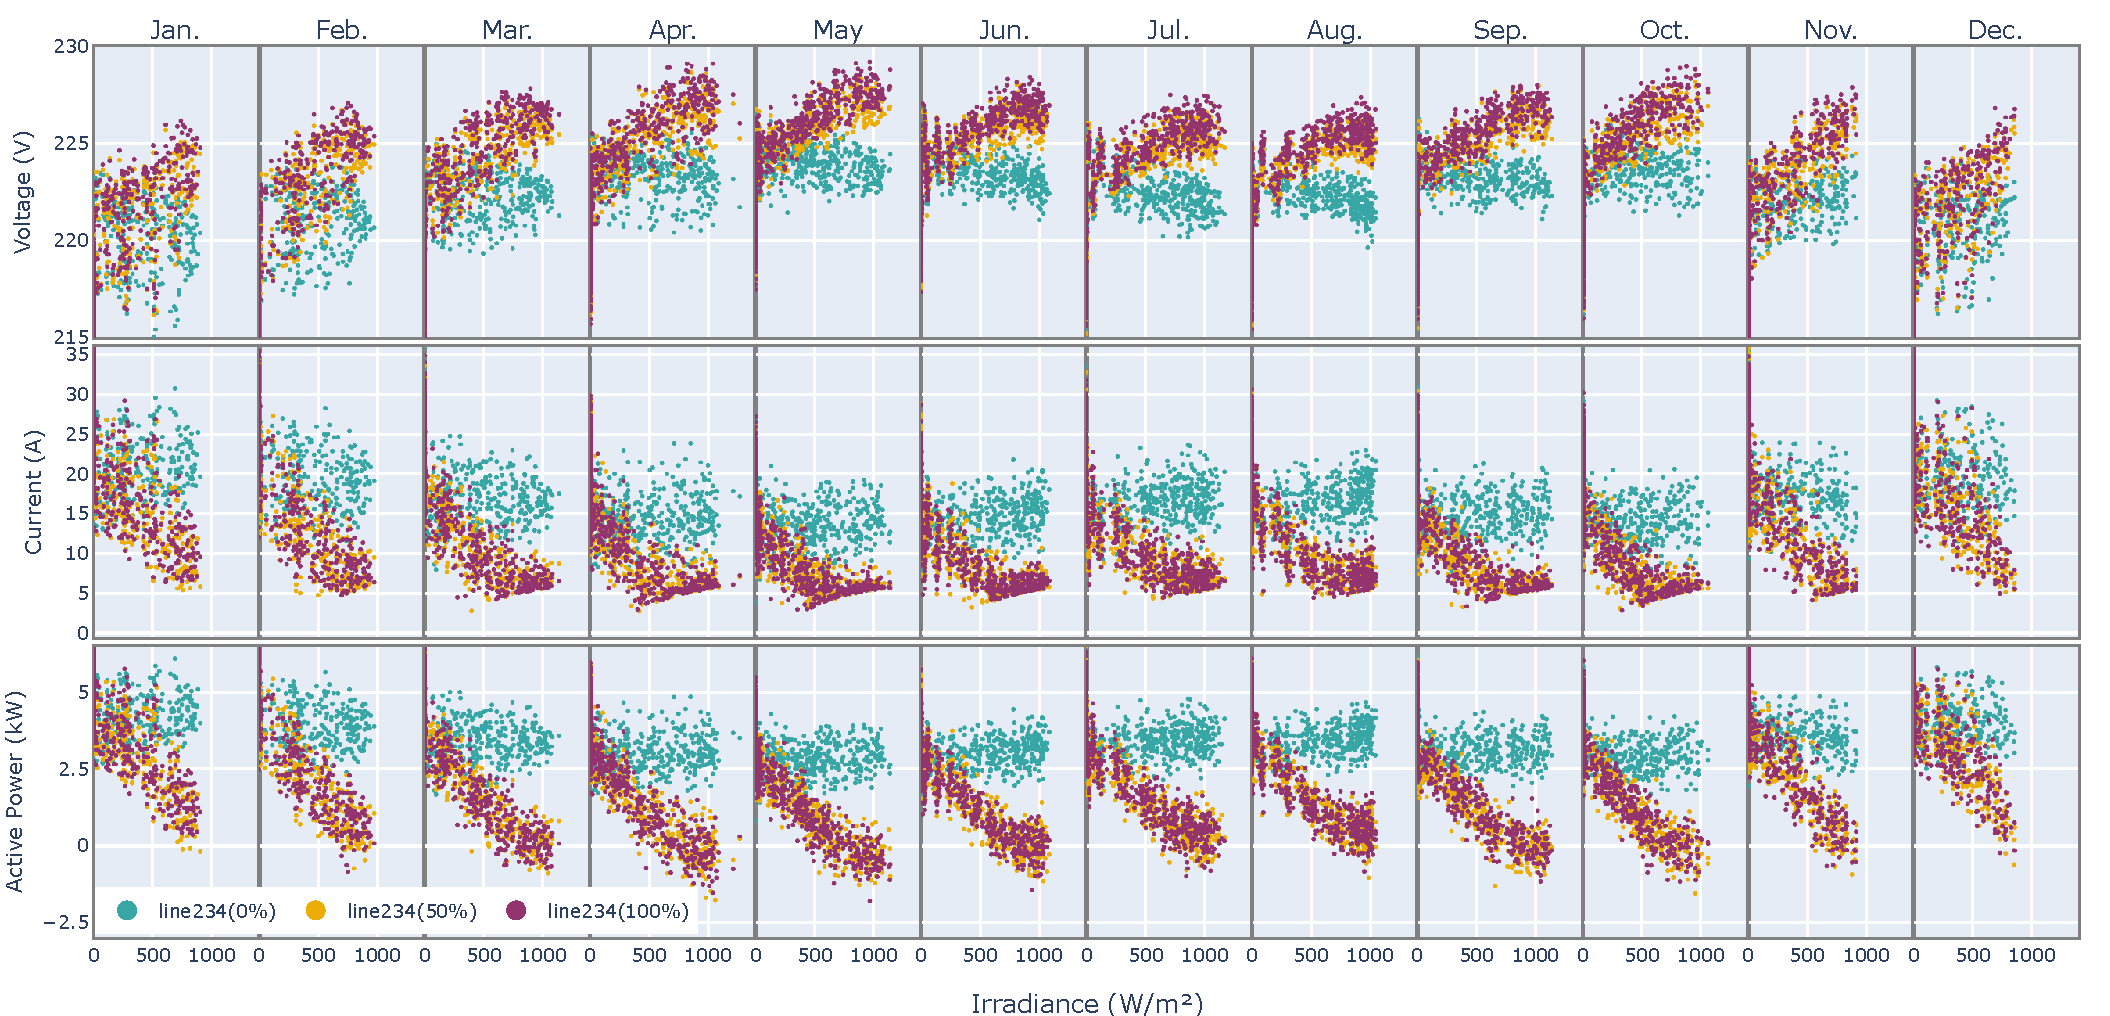
\includegraphics[height=0.7\textheight]{../figs/S_VIP_Irr_line234.pdf}
\end{center}
\end{frame}

\begin{frame}[label={sec:org70b93b5}]{Los Sistemas Fotovoltaicos y la Red Eléctrica}
\begin{itemize}
\item Las rampas de potencia debidas a las fluctuaciones de radiación
solar pueden entorpecer el adecuado funcionamiento de los equipos
conectados a la red y los elementos de protección existentes.

\begin{center}
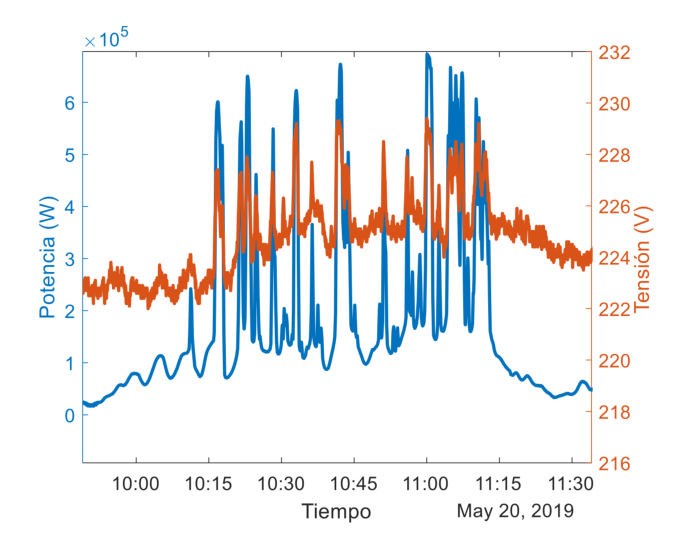
\includegraphics[height=0.75\textheight]{../figs/VariacionTension_RampasPotencia.pdf}
\end{center}
\end{itemize}
\end{frame}


\begin{frame}[label={sec:org1b4459c}]{Los Sistemas Fotovoltaicos y la Red Eléctrica}
\begin{itemize}
\item Los SFCR pueden proporcionar servicios de apoyo a la red gracias a
las funcionalidades que incorporan los inversores de conexión a red,
capaces de controlar la potencia activa inyectada en el punto de
conexión, y la potencia reactiva en funcionamiento normal o para
enfrentarse a huecos de tensión.

\begin{center}
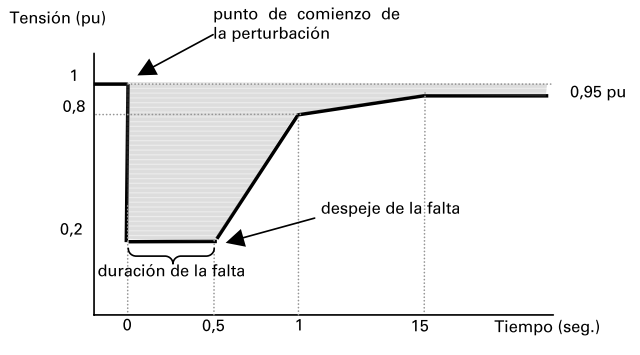
\includegraphics[height=0.7\textheight]{../figs/hueco-tension.png}
\end{center}
\end{itemize}
\end{frame}

\begin{frame}[label={sec:orgd1705aa}]{Variabilidad de la Radiación}
\begin{itemize}
\item La irradiancia solar es un proceso con inercia y con baja
probabilidad para mostrar cambios abruptos.

\item La probabilidad de ocurrencia de fluctuaciones elevadas es
sustancialmente menor al observar con resoluciones temporales
altas.
\end{itemize}

\begin{center}
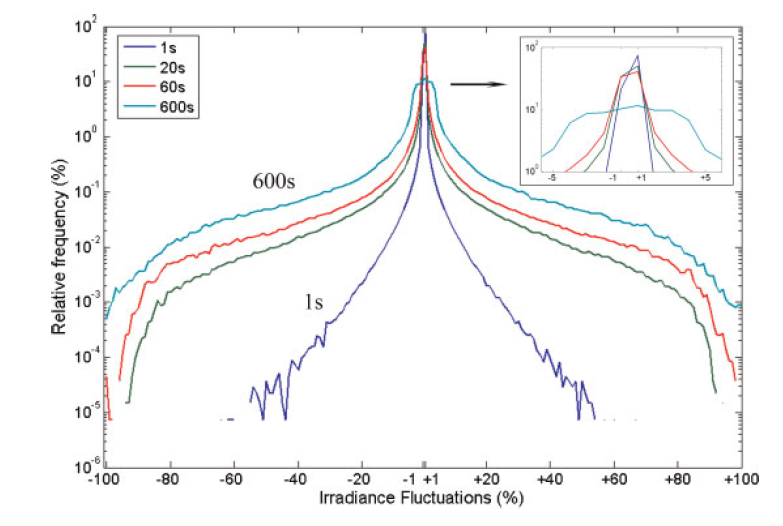
\includegraphics[height=0.65\textheight]{../figs/FluctuacionIrradiancia_Marcosetal2011.png}
\end{center}
\end{frame}

\begin{frame}[label={sec:orgf2f0f8c}]{Variabilidad de la Radiación}
\begin{itemize}
\item El nivel de fluctuación depende del comportamiento de la atmósfera (mayor en días parcialmente cubiertos).
\end{itemize}

\begin{center}
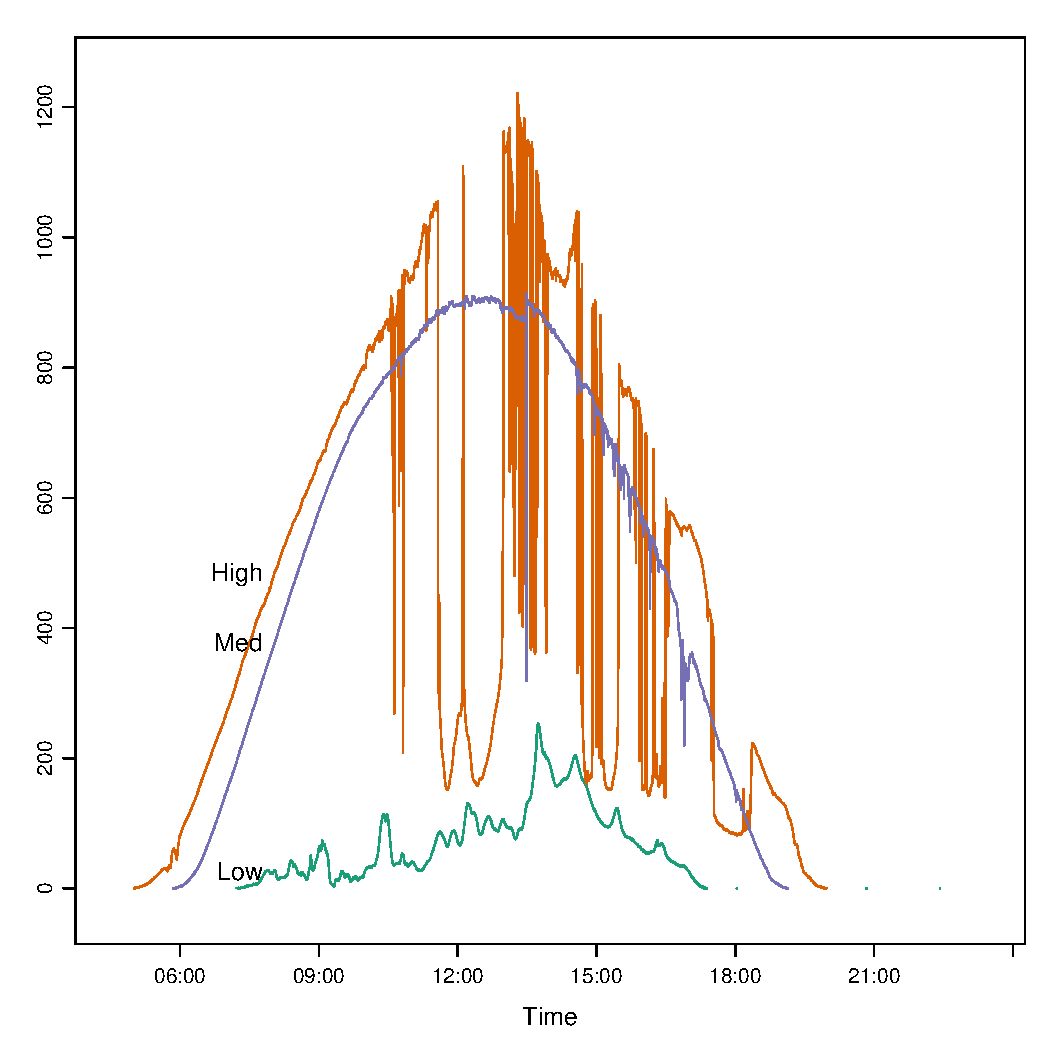
\includegraphics[height=0.8\textheight]{../figs/radLowMedHigh.pdf}
\end{center}
\end{frame}


\section{Incertidumbre y Predicción}
\label{sec:org16bb8bb}

\begin{frame}[label={sec:orgcf41d63}]{Generación y Demanda}
La \alert{casación entre generación y demanda} que se consigue en las redes
eléctricas se basa en la \alert{programación} de las diferentes unidades de
\alert{generación} disponibles para suministrar la \alert{demanda prevista} y para
constituir \alert{reservas} que hagan frente a las posibles \alert{variaciones} en la
demanda.

\begin{center}
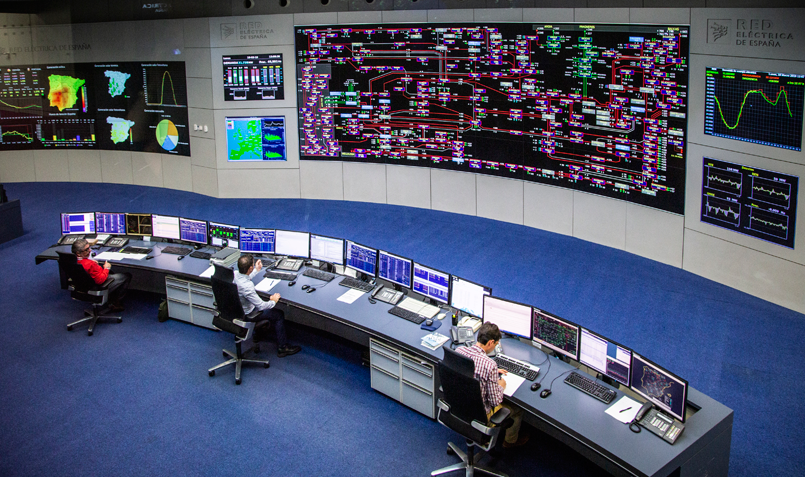
\includegraphics[height=0.65\textheight]{../figs/CentroOperacionesREE.png}
\end{center}
\end{frame}


\begin{frame}[label={sec:org7053c79}]{Programación de la generación}
Esta programación se produce en \alert{escalas y horizontes temporales diversos} y se \alert{actualiza de forma sistemática} de acuerdo con las variaciones previstas en la predicción de la demanda.

\begin{center}
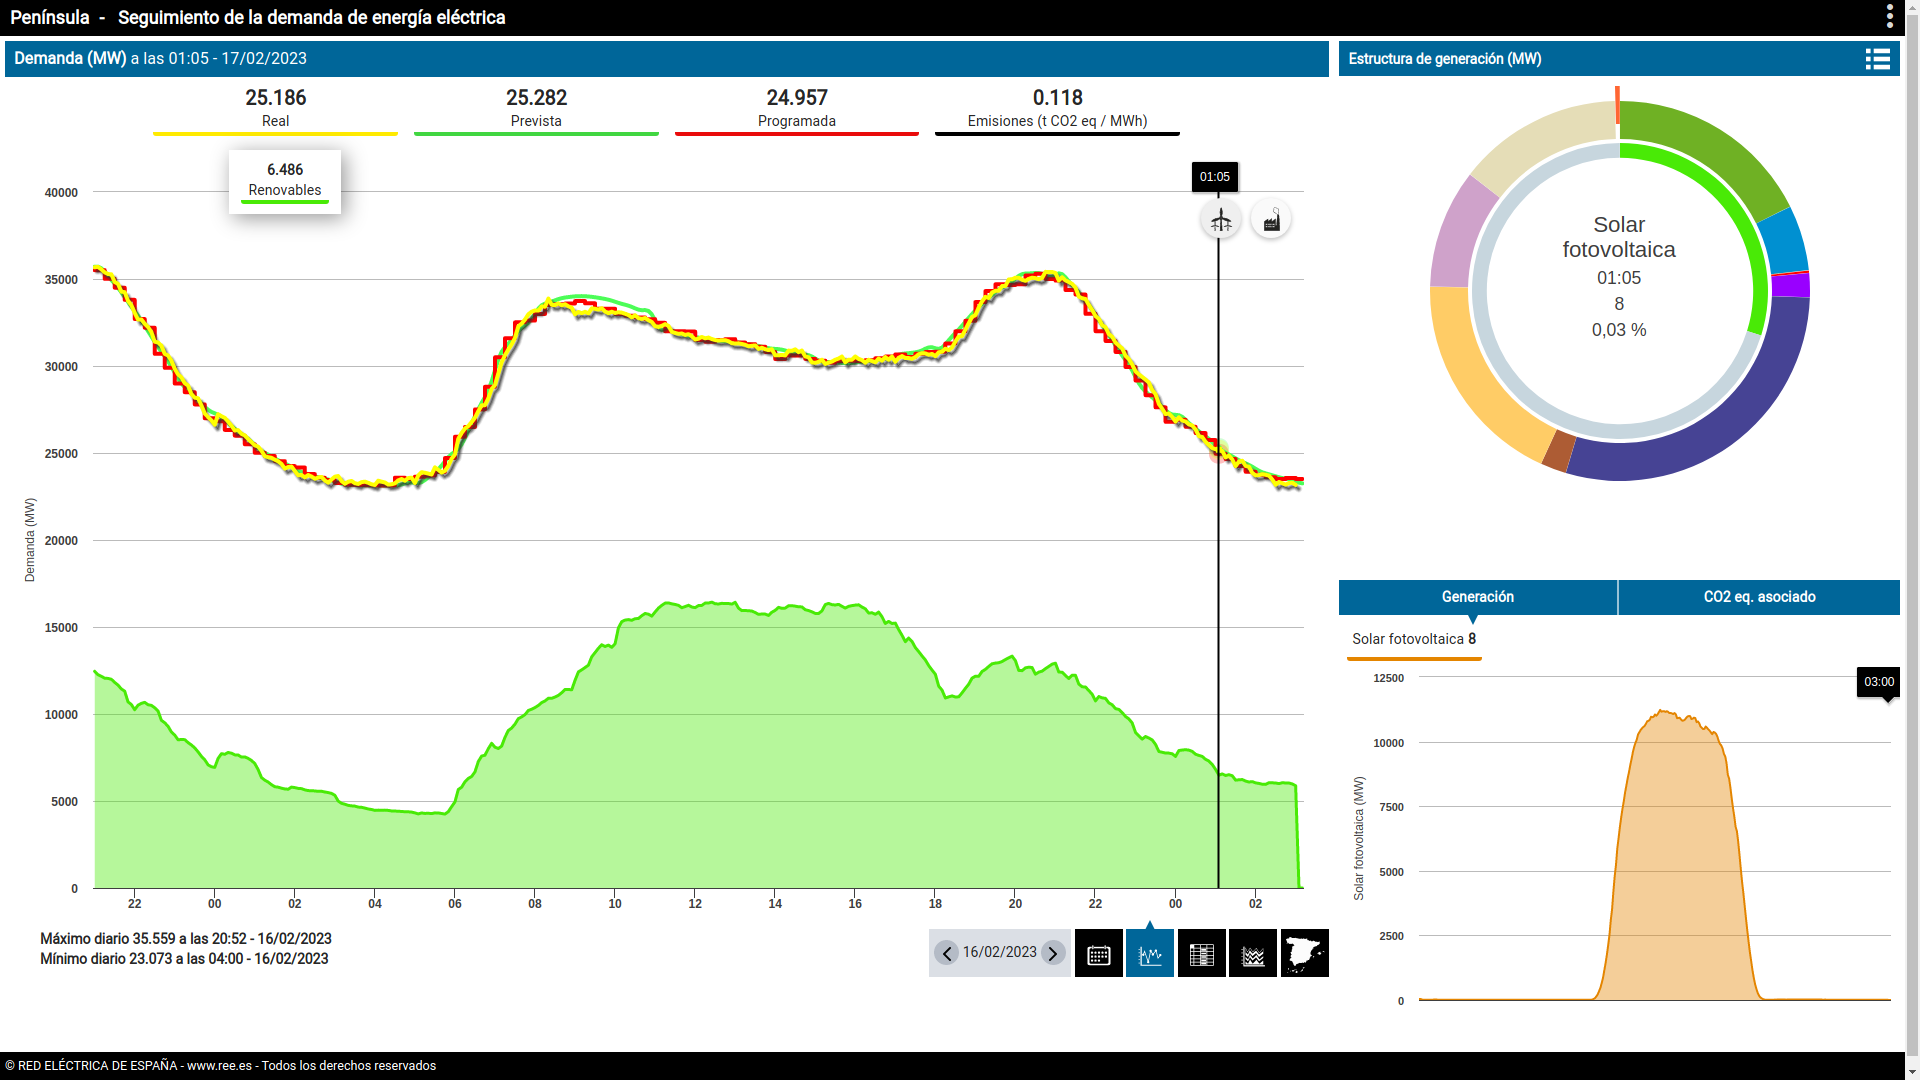
\includegraphics[height=0.6\textheight]{../figs/CurvaDemandaREE.png}
\end{center}

\begin{center}
\url{https://demanda.ree.es/visiona/peninsula/demandaqh/total/}
\end{center}
\end{frame}


\begin{frame}[label={sec:orgb03e95c}]{Participación masiva de la fotovoltaica}
La \alert{inclusión masiva} de sistemas fotovoltaicos en la red \alert{modifica el
equilibrio} existente y puede implicar el uso de las reservas de
generación previstas originalmente para asumir las variaciones de la
demanda.

\begin{center}
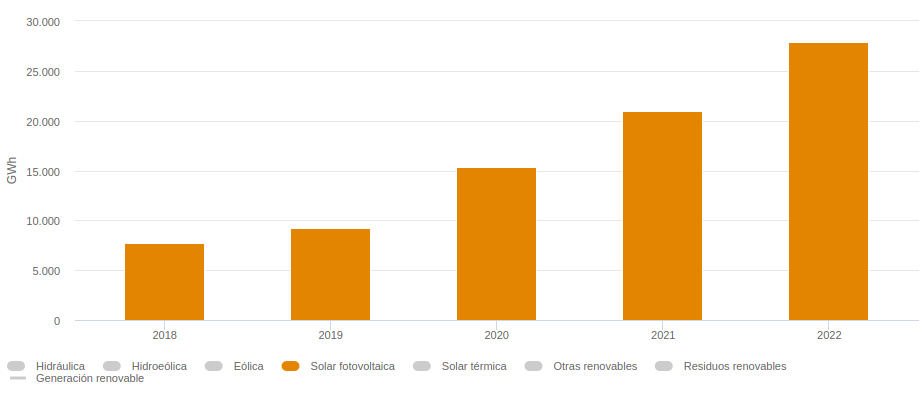
\includegraphics[height=0.6\textheight]{../figs/EvolucionGeneracionFV_REE.png}
\end{center}
\end{frame}


\begin{frame}[label={sec:org575f541}]{Predicción de la Potencia}
En este contexto el reto no es tanto la variabilidad como la
\alert{predicción}:

\begin{itemize}
\item La realización de predicciones en horizontes horarios o diarios de
la potencia generada por un sistema fotovoltaico o por un grupo de
sistemas es crucial para facilitar la integración de sistemas
fotovoltaicos en redes eléctricas.

\item La predicción de radiación solar y potencia de sistemas
fotovoltaicos es un área de investigación de plena actualidad.
\end{itemize}
\end{frame}

\begin{frame}[label={sec:org58195c0}]{Ejemplo: proyecto europeo PVCROPS}
\begin{itemize}
\item Herramienta de aprendizaje automático o \emph{machine learning}
entrenada con series históricas de predicciones NWP y medidas de
potencia eléctrica (30 días en la serie temporal de
entrenamiento).
\item Predicción de potencia AC con resolución horaria y un horizonte
temporal de 1 día.
\end{itemize}


\begin{center}
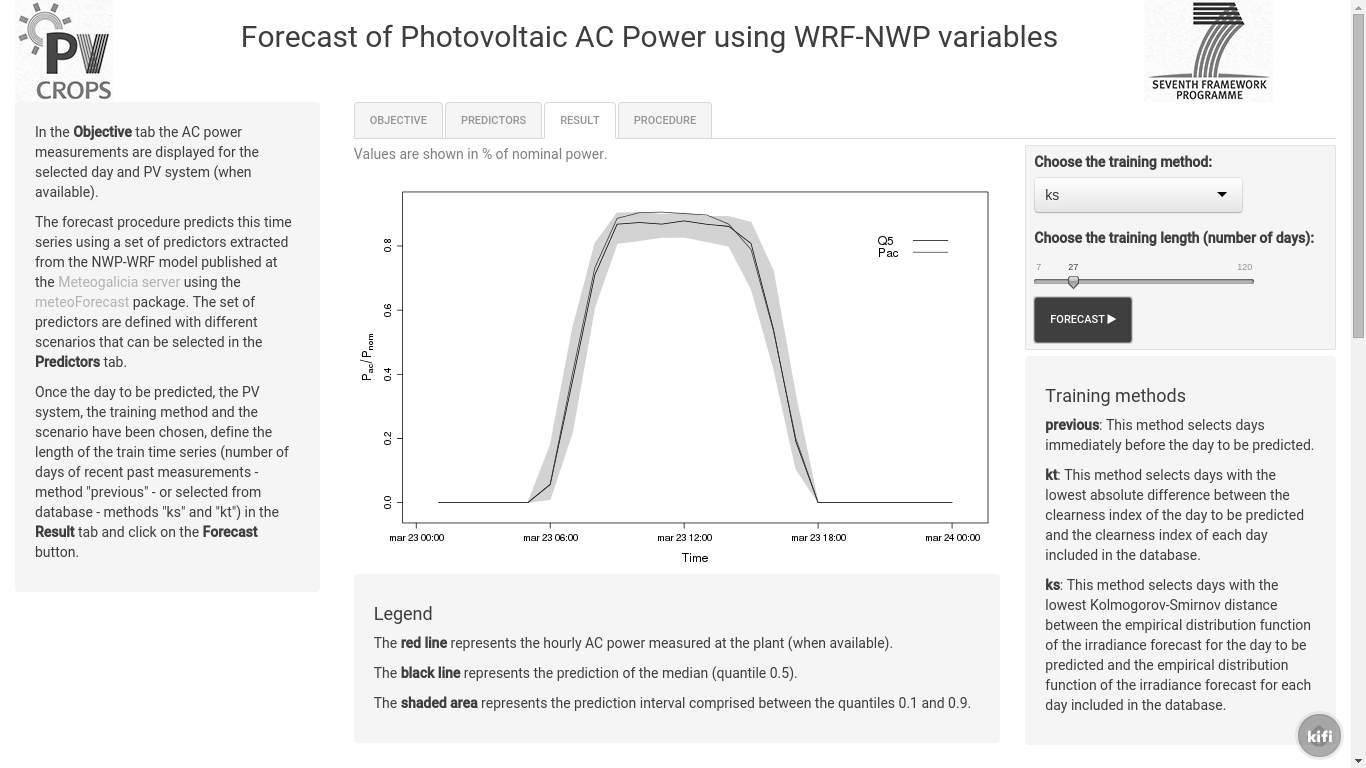
\includegraphics[height=0.65\textheight]{../figs/ForecastShiny.png}
\end{center}
\end{frame}

\begin{frame}[label={sec:org6b61eaa}]{Ejemplo: proyecto europeo PVCROPS}
Se emplean como entradas las predicciones de variables
meteorológicas generadas por modelos de predicción meteorológica
numérica e índices de variación espacial y temporal estimados con
las variables meteorológicas.

\begin{center}
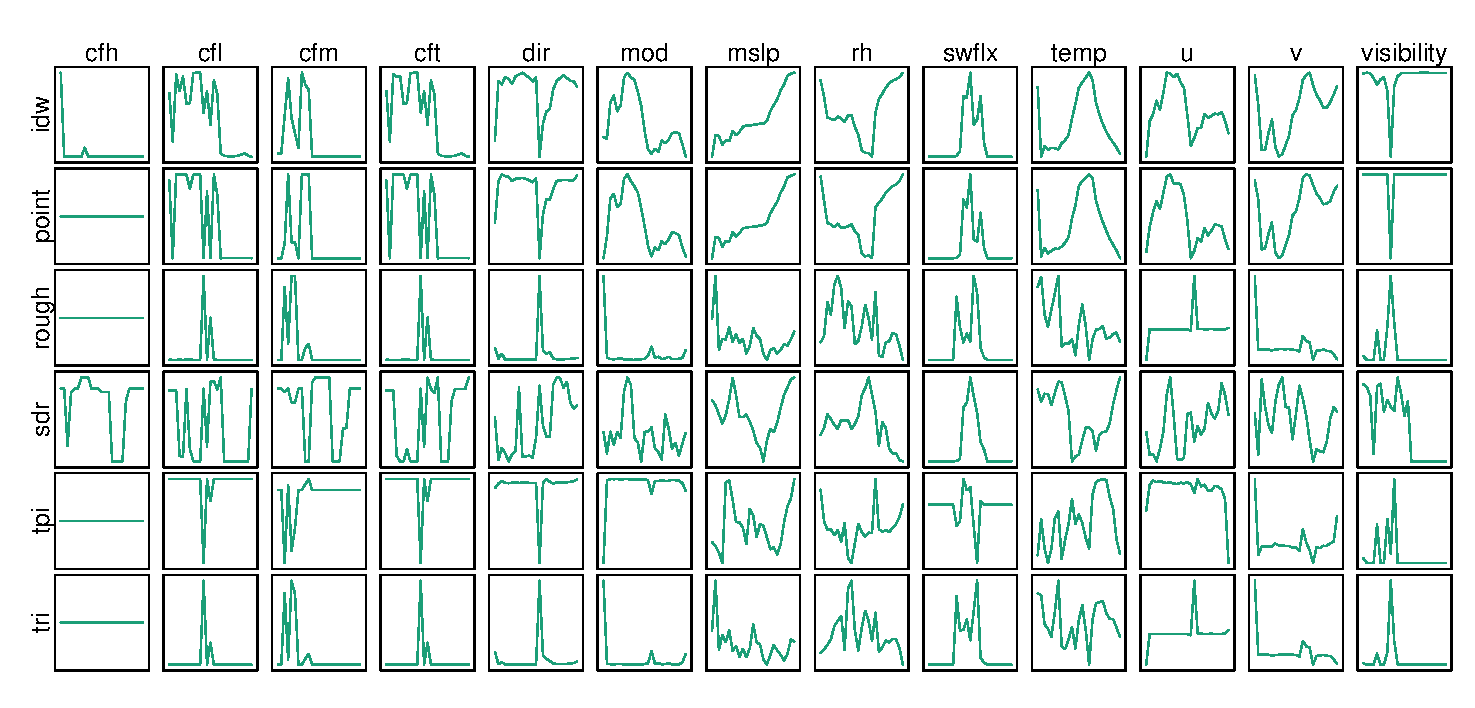
\includegraphics[height=0.7\textheight]{../figs/varsComplete.pdf}
\end{center}
\end{frame}


\begin{frame}[label={sec:orgee86a58}]{Ejemplo: proyecto europeo PVCROPS}
Genera predicciones probabilísticas, entregando tanto la mediana de la
predicción como un intervalo de confianza, que permite cuantificar la
fiabilidad de la predicción, y que puede servir como medida indirecta
de la variabilidad futura.

\begin{center}
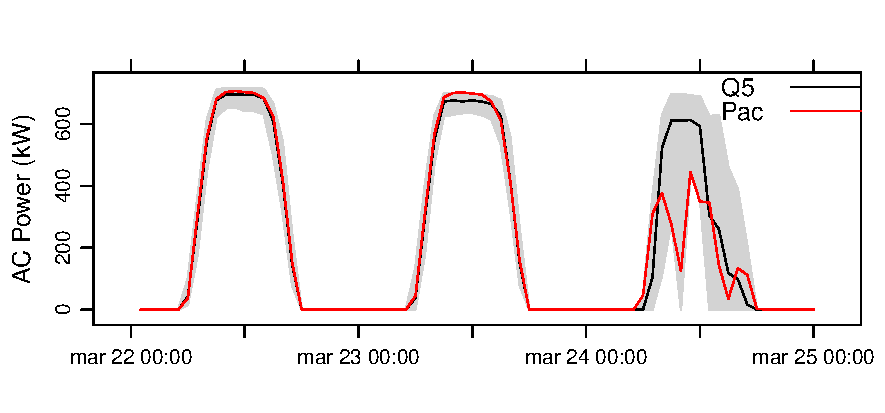
\includegraphics[width=0.6\textwidth]{../figs/powerResult.pdf}
\end{center}

\begin{center}
\url{http://vps156.cesvima.upm.es:3838/predictPac/}
\end{center}
\end{frame}


\begin{frame}[label={sec:orgb040857}]{Predicciones agregadas}
Las predicciones obtenidas mejoran cuando las predicciones se aplican
a un conjunto de sistemas.
\end{frame}

\section{Variabilidad de la Potencia}
\label{sec:orgf24b87b}

\begin{frame}[label={sec:org76432f9}]{Variabilidad Conjunta}
La variabilidad presente en la irradiancia solar se \alert{atenúa} en la potencia AC:
\begin{itemize}
\item por la \alert{dispersión} espacial \alert{entre diferentes centrales}.
\item por la \alert{dispersión} espacial \alert{dentro de una central}.
\end{itemize}
\end{frame}

\begin{frame}[label={sec:orgd2d3202}]{Dispersión espacial entre centrales}
\begin{itemize}
\item En términos generales, la \alert{dispersión espacial de sistemas
fotovoltaicos diferentes} conectados a la misma red \alert{atenúa} la
variabilidad conjunta.

\begin{center}
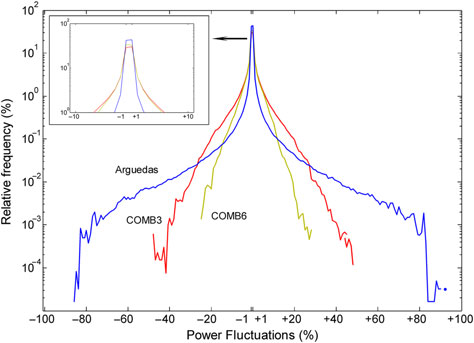
\includegraphics[height=0.5\textheight]{../figs/Variabilidad_DispersionGeografica_Plantas.png}
\end{center}

\item El \alert{nivel de atenuación depende} principalmente de las
\alert{características meteorológicas} de la zona y época, y de la
\alert{distancia} entre los sistemas.

\item Para \alert{distancias mayores de \(\SI{5}{\kilo\meter}\)} las fluctuaciones
de irradiancia con resolución temporal de 1 minuto están
esencialmente \alert{incorreladas}.
\end{itemize}
\end{frame}

\begin{frame}[label={sec:org8ef2a40}]{Dispersión espacial dentro de una central}
En términos generales, la \alert{dispersión espacial} de generadores
fotovoltaicos pertenecientes a \alert{una misma central} \alert{atenúa} la
variabilidad conjunta.

\begin{center}
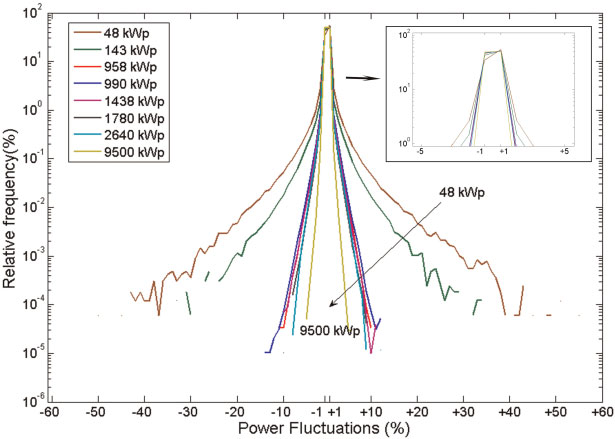
\includegraphics[height=0.7\textheight]{../figs/Variabilidad_DispersionGeografica_Planta.png}
\end{center}
\end{frame}

\begin{frame}[label={sec:org20c95ab}]{Dispersión espacial dentro de una central}
La correlación entre la potencia de cada inversor \alert{depende} de la \alert{resolución temporal}, la \alert{distancia} entre los inversores, y el \alert{nivel de fluctuación del día} en cuestión.

\begin{center}
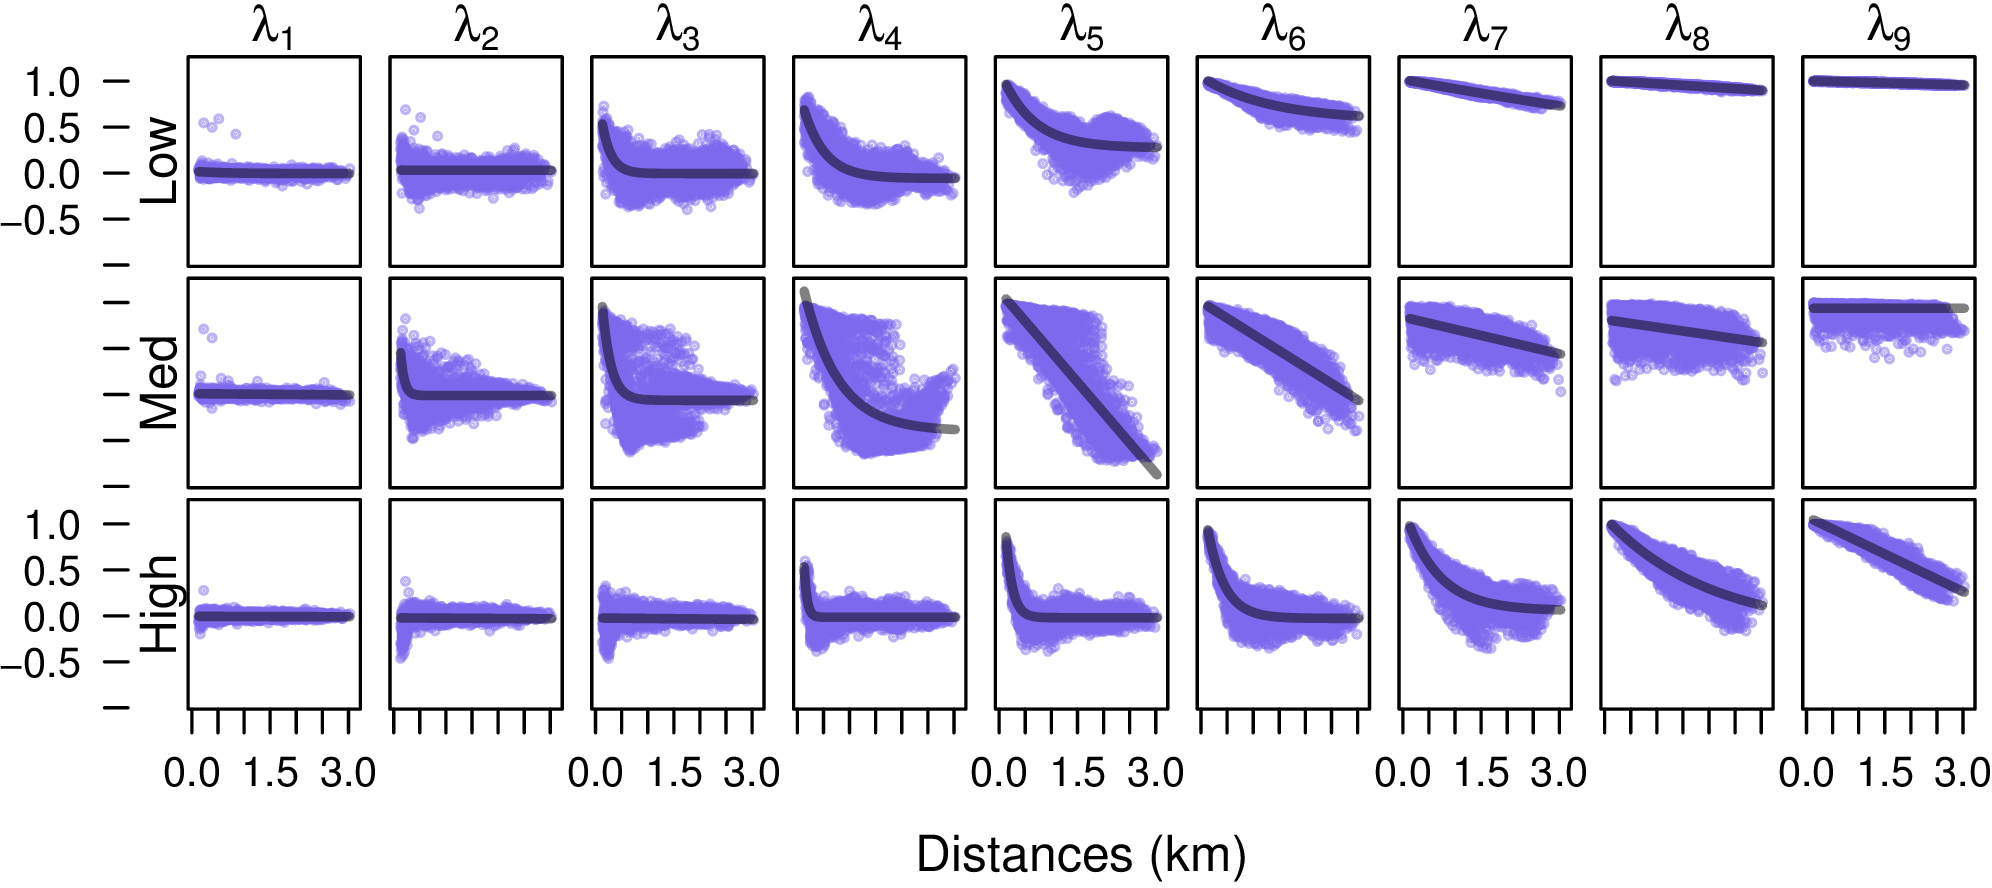
\includegraphics[height=0.6\textheight]{../figs/corDistMatrix_nls.png}
\end{center}
\end{frame}

\begin{frame}[label={sec:org5b288a0}]{Dispersión espacial dentro de una central}
Escalas temporales bajas (\(\tau <\qty{1}{\min}\)): correlaciones bajas.

\begin{center}
  \begin{tikzpicture}
    \node[anchor=south west,inner sep=0] at (0,0) {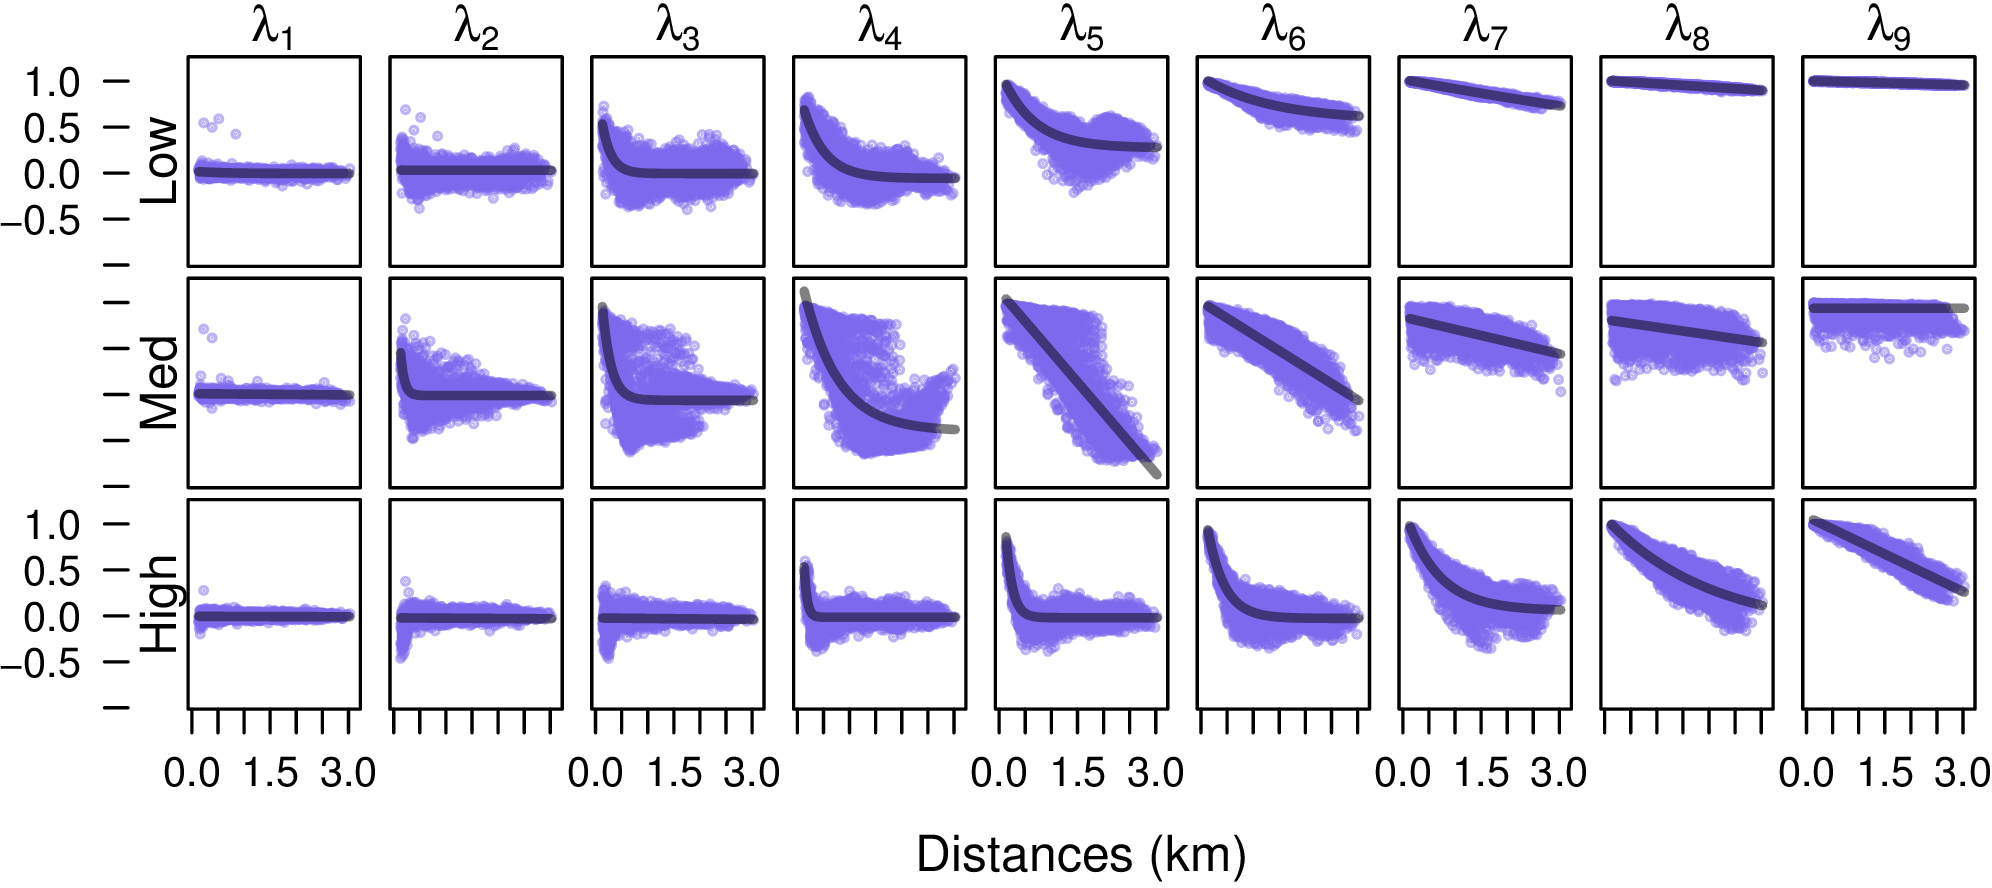
\includegraphics[height=0.5\textheight]{../figs/corDistMatrix_nls.png}};
      \draw[red,ultra thick,rounded corners] (0,0) rectangle (3, 0.55\textheight);
    \end{tikzpicture}
  \end{center}
\end{frame}

\begin{frame}[label={sec:org9fb3fff}]{Dispersión espacial dentro de una central}
Escalas temporales intermedias: la correlación depende fuertemente del nivel de fluctuación diario.

\begin{center}
  \begin{tikzpicture}
    \node[anchor=south west,inner sep=0] at (0,0) {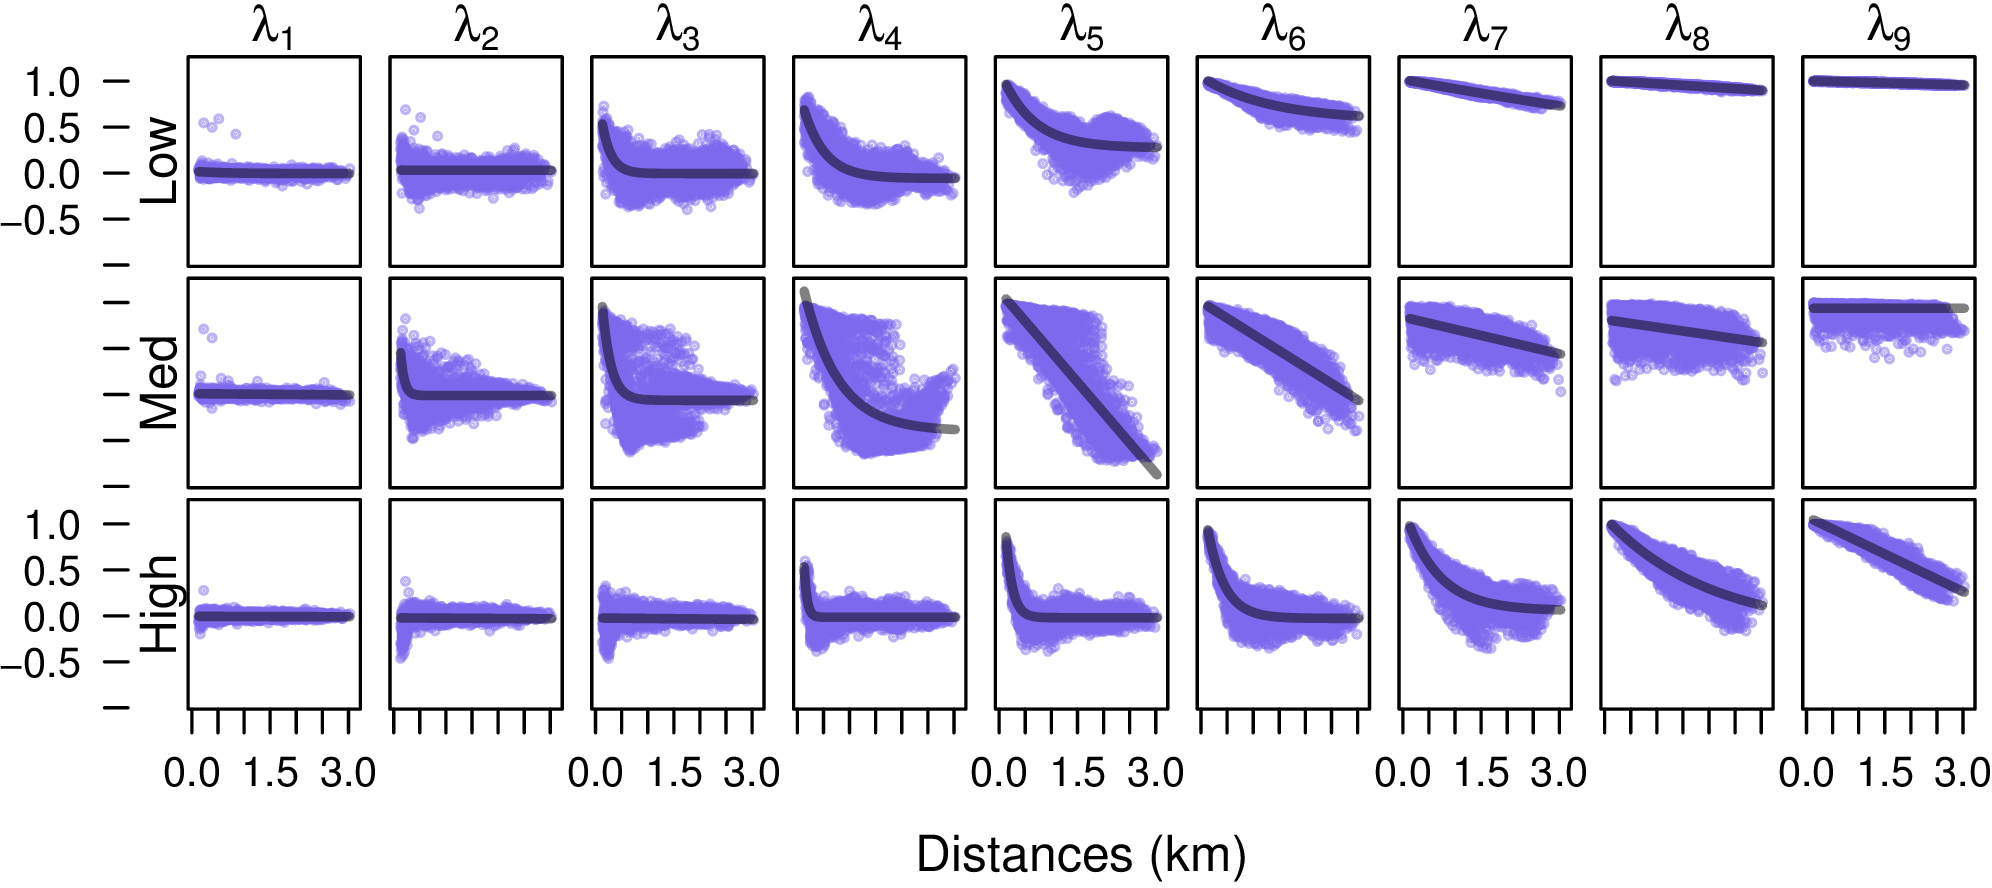
\includegraphics[height=0.5\textheight]{../figs/corDistMatrix_nls.png}};
      \draw[red,ultra thick,rounded corners] (2.6,0) rectangle (7, 0.55\textheight);
    \end{tikzpicture}
  \end{center}
\end{frame}

\begin{frame}[label={sec:orgc4ad31b}]{Dispersión espacial dentro de una central}
Escalas temporales altas, \(\tau > \qty{20}{\min}\): correlaciones altas y positivas que decrecen de forma exponencial con la distancia; clara dependencia con el nivel de fluctuación diaria.

\begin{center}
  \begin{tikzpicture}
    \node[anchor=south west,inner sep=0] at (0,0) {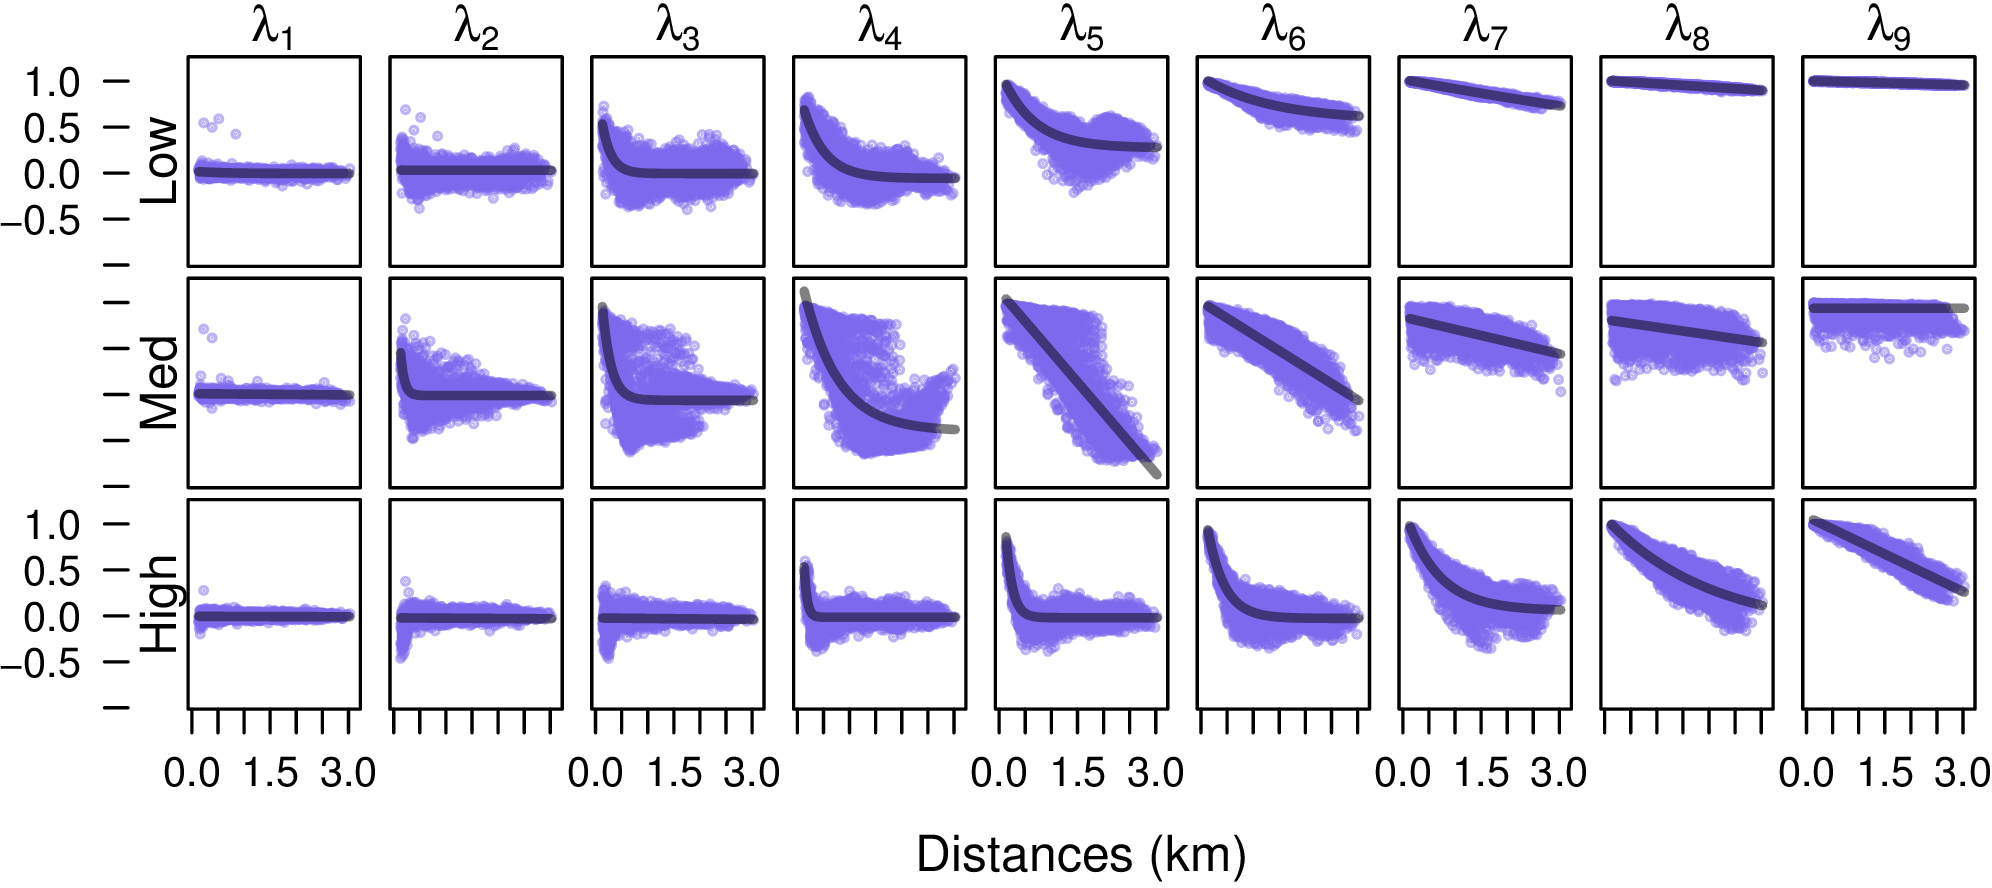
\includegraphics[height=0.5\textheight]{../figs/corDistMatrix_nls.png}};
      \draw[red,ultra thick,rounded corners] (6.5,0) rectangle (10, 0.55\textheight);
    \end{tikzpicture}
  \end{center}
\end{frame}

\begin{frame}[label={sec:org4a40ee1}]{Normativas de red}
\begin{itemize}
\item La variabilidad en escalas de tiempo bajas puede influir en mayor o
menor medida en el funcionamiento de la red eléctrica.
\item Existencia de normativas y recomendaciones para la integración de
sistemas fotovoltaicos en la red.
\item Ejemplo clásico: Autoridad Eléctrica de Puerto Rico incluye en su
normativa el concepto de rampa para cuantificar las fluctuaciones
admisibles:
\end{itemize}

\begin{quote}
A 10\% per minute rate (based on AC contracted capacity) limitation shall be enforced. This ramp rate limit applies both to the increase and decrease of power output and is independent of meteorological conditions.
\end{quote}
\end{frame}

\begin{frame}[label={sec:org95a4697}]{Definiciones de rampas}
Uno de los problemas principales en este requerimiento (y otros similares) es que, aunque es fácil identificar visualmente una rampa en una serie temporal de potencia, no existe consenso en una definición formal que permita identificarla y cuantificarla.
\end{frame}

\begin{frame}[label={sec:orgb4ee010}]{Ejemplos de definiciones de rampas}
\begin{itemize}
\item Existe una rampa al inicio de un intervalo temporal si la magnitud del cambio en un instante temporal posterior es mayor que un umbral predeterminado.
\end{itemize}
\[ 
\left| P(t +\Delta_t) - P(t)\right| > \tau
\]

\begin{itemize}
\item Existe una rampa en un intervalo temporal si la diferencia entre los
valores máximo y mínimo supera un determinado umbral.
\end{itemize}
\[
\max(\{P_t: t = t_0, \dots, t_0+\Delta_t\}) - \min(\{P_t: t=t_0,
\dots, t_0+\Delta_t\}) > \tau
\]

\begin{itemize}
\item Existe una rampa dentro de un intervalo si el ratio entre el valor absoluto de la diferencia entre las medidas de potencia en dos instantes temporales, y la longitud del intervalo supera un determinado umbral.
\end{itemize}
\[
\frac{\left|P(t + \Delta_t) - P(t)\right|}{\Delta_t} > \tau
\]

\begin{itemize}
\item Existe una rampa en un intervalo si el valor absoluto de la señal de diferencias filtrada (por ejemplo, mediante una media móvil) supera un determinado umbral.
\end{itemize}
\end{frame}

\begin{frame}[label={sec:orgdd89c28}]{Limitación de rampas}
La limitación de las rampas de los sistemas fotovoltaicos es un
requerimiento que se debe afrontar, principalmente en el caso de las
centrales fotovoltaicas de gran tamaño.

Existen tres estrategias principales:
\begin{itemize}
\item el uso de sistemas de acumulación energética;
\item acumulación energética combinada con predicción de rampas;
\item predicción de rampas sin acumulación.
\end{itemize}
\end{frame}

\begin{frame}[label={sec:org2f9138b}]{Limitación de rampas}
\begin{itemize}
\item La inclusión de sistemas de acumulación, siendo la opción más
evidente en centrales de gran tamaño, conlleva aumentos en los
costes de instalación y en la complejidad y mantenimiento del
sistema.

\item Las herramientas de predicción de rampas combinadas con mecanismos
de control en el inversor fotovoltaico permiten reducir el tamaño de
la acumulación necesaria, e incluso se puede evitar su inclusión en
determinadas combinaciones de potencia instalada y requerimientos de
rampas admisibles.
\end{itemize}
\end{frame}
\begin{frame}[label={sec:org77e05d2}]{Cálculo de sistema de acumulación}
La batería es un elemento caro.

Objetivos:
\begin{itemize}
\item Dimensionar, en potencia y energía, la batería mínima necesaria.
\item Desarrollar estrategias de gestión que permitan, cumpliendo con la rampa máxima, minimizar el coste de la energía (LCOE):
\begin{itemize}
\item Minimizar Batería
\item Minimizar Degradación
\item Minimizar Pérdidas
\end{itemize}
\end{itemize}

¿Cuánto almacenamiento es necesario para cumplir con una limitación de
rampa? Modelo de la peor fluctuación
\end{frame}
\end{document}